%%%%%%%%%%%%%%%%%%%%%%%%%%%%%%%%%%%%%%%%%%%%%%%%%%%%%%%%%%%%%%%%%%%%%%%%%%%%%%%
%% Outline
%%%%%%%%%%%%%%%%%%%%%%%%%%%%%%%%%%%%%%%%%%%%%%%%%%%%%%%%%%%%%%%%%%%%%%%%%%%%%%%
% 
% Explain problem without timing details. Use figure that has turn lengths with 
% no offsets. Show a packet traversing through path with latencies outlined and 
% the packet getting delayed. Explain figure.
% 
% Though the l3 hit path is simple, whole l2 miss path is a nontrivial problem 
% - many tradeoffs, used linear optimization. Wrote simulator to explore this.  
%   Ultimately found a general scheme
% that an optimizer couldn't beat for the l3 miss path. Finding agood balance 
% between
% the hit and miss paths required an optimizer and we did not find a general 
% scheme
% 
% \subsection{L2 Miss Timing Sequence}
% Introduce l3 hit timing sequence with figure. Explain figure.
% 
% Show l3 miss timing sequence. Use figure.
% 
% \subsection{Latency Simulator \& Optimal Coordination}
% 
% Explain goal of coordinating (EV of L2 miss latency). Usually achieved by 
% aligning turns of adjacent devices. Use turn lengths (duration a TC is 
% scheduled to use a device - depends time to send message, affects 
% ``randomness'' of schedule) and offsets (difference in start times that
% improves how the schedule relates to the schedule of other devices).
% 
% Show how to optimize l3 hits. Use figure.
% 
% Explain tradeoffs. Use figure?? It is not simple to solve.
% 
% Wrote our own l2 miss (l2 to l2) timing simulator. Explain what it simulates.  
% (Assumes uniform random arrival, calculate latency for every possible arrival 
% in a schedule, gets EV of latency).
% 
% Exhaustive search of L3 hit path. Confirms that an intuitive design is best.
% 
% Cannot exhaustively search L3 miss path latencies. Instead use linear 
% optimizatin. Search space has many relative minima (change offset slightly, 
% suddenly schedule is much better) - cannot use hill climbing. Use simulated 
% annealing. Explain our simulated annealing implementation. Optimize for l3 
% miss alone and l2 miss latency assuming hit rate of 90\%.
% 
% Tried a scheme we suspected would have a good L3 miss latency. Optimal result 
% was different. Adjusted optimizer result to something that made more 
% intuitive sense and iterated. Reran optimizer on result of iterative 
% approach, and the optimizer could not find a better scheme in 20,000 steps.
% 
% Explain optimal scheme. Use figure.
% 
% For l2 miss latency, no intuitive general approach could be found. Balance 
% between hit/miss paths is difficult.


%%%%%%%%%%%%%%%%%%%%%%%%%%%%%%%%%%%%%%%%%%%%%%%%%%%%%%%%%%%%%%%%%%%%%%%%%%%%%%%
%% Old Figures
%%%%%%%%%%%%%%%%%%%%%%%%%%%%%%%%%%%%%%%%%%%%%%%%%%%%%%%%%%%%%%%%%%%%%%%%%%%%%%%
% \begin{figure}
%     \begin{center}
%         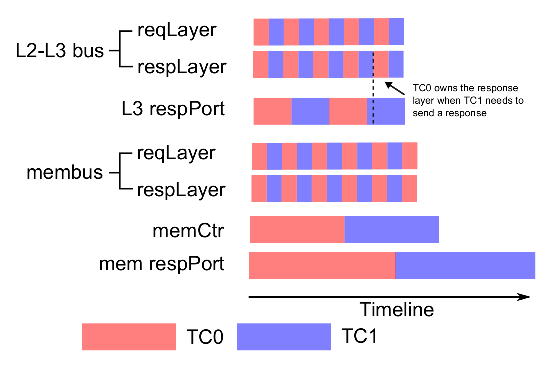
\includegraphics[width=3.46in]{figs/baseline_schedule.eps}
%         \caption{Cache hit timing sequence.}
%         \label{fig:naive_scheme}
%     \end{center}
% \end{figure}
% 
% 
% \begin{figure}
%     \begin{center}
%         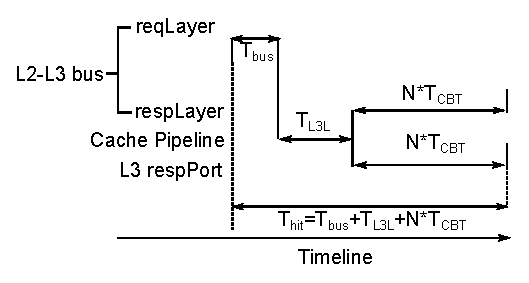
\includegraphics[width=2.4675in]{figs/hit_timing.eps}
%         \caption{L3 cache hit timing sequence.}
%         \label{fig:hit_timing}
%     \end{center}
% \end{figure}
% 
% \begin{figure}
%     \begin{center}
%         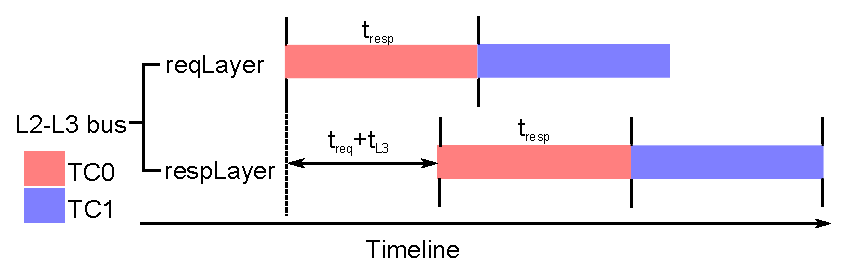
\includegraphics[width=3.2624in]{figs/hit_schedule.eps}
%         \caption{Cache hit timing path schedule.}
%         \label{fig:hit_schedule}
%     \end{center}
% \end{figure}
% 
% \begin{figure}
%     \begin{center}
%         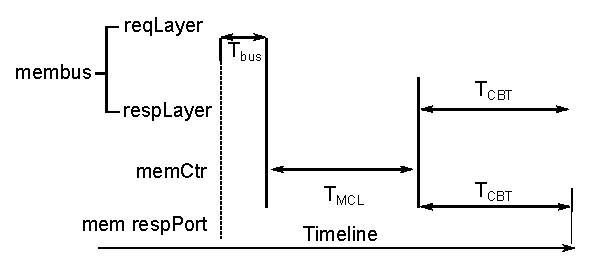
\includegraphics[width=2.9475in]{figs/miss_timing.eps}
%         \caption{The L3-memory timing sequence.}
%         \label{fig:miss_timing}
%     \end{center}
% \end{figure}
% 
% \begin{figure}
%     \begin{center}
%         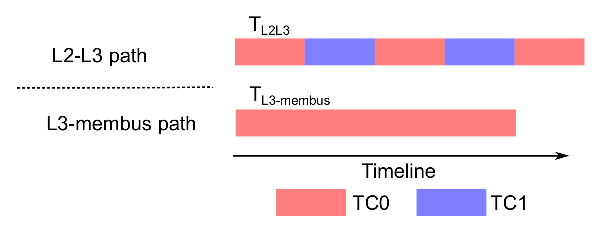
\includegraphics[width=2.9475in]{figs/coordination.eps}
%         \caption{A coordinated cache miss path schedule.}
%         \label{fig:coordination}
%     \end{center}
% \end{figure}

\section{Time Slice Coordination}
\label{sec:coordination}
The Timing Compartments architecture relies heavily on time multiplexing to 
protect shared resources including the L2-L3 bus, the L3-memory bus, and the 
memory controller. These resources frequently interact since each is involved 
in handling L2 misses. If the time multiplexing schedules for each of these 
resources are not designed to account for this interaction, it could lead to 
exorbitant latencies and wasted bandwidth.

\begin{figure}
    \begin{center}
        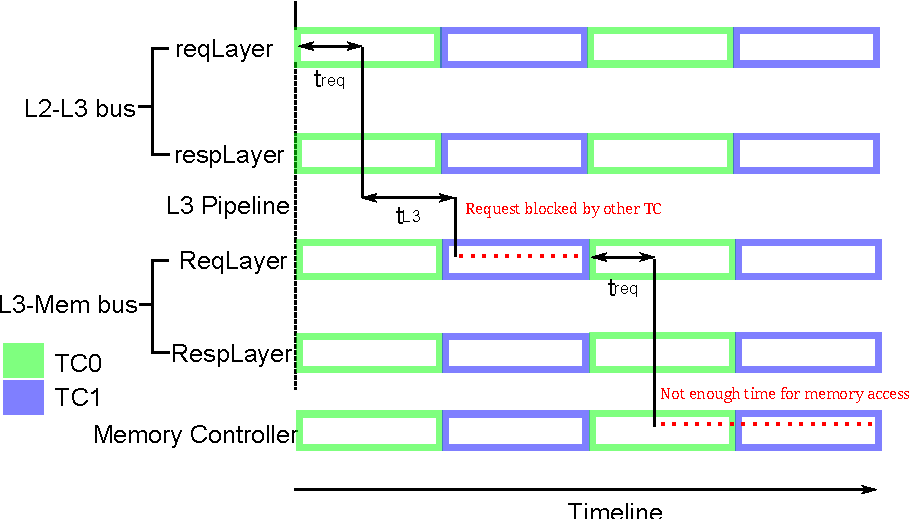
\includegraphics[width=3.5in]{figs/problem.pdf}
        \caption{A poorly performing time multiplexing schedule.}
        \label{fig:problem}
    \end{center}
\end{figure}

Figure \ref{fig:problem}, illustrates the problem. It shows when each of two 
timing compartments are scheduled to use the time multiplexed resources along 
the L2 miss path. Green blocks indicate that TC0 is scheduled to use the device, 
and blue blocks indicate that TC1 is scheduled. We refer to the block of time 
that a timing compartment is scheduled to use a device as the \emph{turn} and 
we refer to the duration of a turn as the \emph{turn length}. In this schedule, 
timing compartments are allotted the same turn length for each time multiplexed 
resource, and the schedule for each device starts at the same time.

%%%%%%%%%%%%%%%%%%%%%%%%%%%%%%%%%%%%%%%%%%%%%%%%%%%%%%%%%%%%%%%%%%%%%%%%%%%%%%%
%% This section is easier to write if we introduce bus layers in the uarch 
%% channel section (section 3)
%%%%%%%%%%%%%%%%%%%%%%%%%%%%%%%%%%%%%%%%%%%%%%%%%%%%%%%%%%%%%%%%%%%%%%%%%%%%%%%
An L3 miss from TC0 is shown proceeding with these time multiplexing schedules.
The miss begins at the L2 request layer where the request is sent to the L3.  
When the L3 access is complete, the request must proceed through the L3-memory 
bus request layer, but at this time TC1 is scheduled to use the L3-memory 
request layer, so it must wait for TC1's turn to finish before the request can 
proceed to the memory controller. Then, when it arrives at the memory 
controller, there is not enough time left in the turn to complete a request, so 
it is blocked again. There are similar issues as the packet traverses the rest
of the path.

Clearly, this schedule is inefficient. When designing a schedule for these 
resources both the L3 hit and L3 miss paths should be considered. In this 
section we describe the timing for both paths. We then show that devising a 
schedule that optimizes just the hit path is straightforward, but scheduling 
the miss path and balancing both is challenging.

\subsection{L2 Miss Timing Paths}
To efficiently time multiplex the resources involved in an L2 miss, 
we must understand the timing of L2 misses. L2 misses take two different 
paths and have different timings depending on whether the L2 miss is an L3 hit 
or miss. This section analyzes L2 miss timings under both cases: an L2 miss
followed by an L3 hit, and an L2 miss followed by an L3 miss.

Figure \ref{fig:hit_timing} shows the timing for an L3 hit. The arrows 
indicate the time that the resource in the corresponding column is used.
The L2 miss begins by transferring a request over the L2-L3 bus request layer 
in $t_{req}$ cycles. Typically, $t_{req}$ depends on how the bus protocol 
requires requests to be sent. The request then arrives at the L3 cache, where 
it takes $t_{L3}$ cycles (i.e. the L3 cache latency). We assume the cache is 
fully pipelined, so even if a request arrives one cycle after another, both can 
use the cache simultaneously, and the access always completes in $t_{L3}$ 
cycles. Finally, the data is transferred from the L3 response port back to the 
L2 over the L2-L3 bus response layer in $t_{resp}$ cycles. Often, $t_{resp}$ 
will be greater than $t_{req}$. It depends on the bus bandwidth and the size of 
a cache block.

\begin{figure}
    \begin{center}
        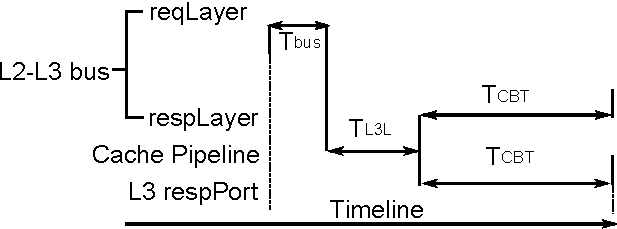
\includegraphics[width=3.5in]{figs/hit_timing.pdf}
        \caption{L3 cache hit timing sequence.}
        \label{fig:hit_timing}
    \end{center}
\end{figure}

Figure \ref{fig:miss_timing} shows the timing for an L3 miss. The request 
begins by transferring over the L2-L3 bus request layer, and similarly takes 
$t_{L3}$ cycles to identify that it is a miss. Afterwards, it sends another 
request to the memory controller over the L3-memory bus request layer in 
$t_{req}$ cycles. Memory requests take variable time to complete, after which 
the data is returned to the L3 in $t_{resp}$ cycles, written to the L3 in 
$t_{L3}$ cycles and finally returned to the L2 after another $t_{resp}$ cycles.

\begin{figure}
    \begin{center}
        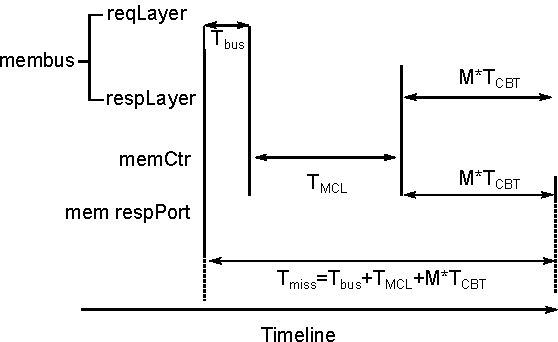
\includegraphics[width=3.5in]{figs/miss_timing.pdf}
        \caption{L3 cache miss timing sequence}
        \label{fig:miss_timing}
    \end{center}
\end{figure}

\subsection{Devising a Schedule}
A good time multiplexing schedule should minimize the L2 miss latency for most 
cases. We can achieve this by controlling the turn lengths and offsets for each 
time multiplexed device. Here, an \emph{offset} refers to a shift in the start 
of the first turn for a single device compared to the start of the full 
schedule.

For a particular resource, suitable turn lengths depend on the latency of that 
resource, and suitable offsets depend on the latency of the preceding resource. 
In other words the turn length should be long enough for the resource's action 
to complete, and the offset should make sure the turn starts when the data is 
available from the preceeding device.

It is also desirable for the schedule to repeat in a short number of cycles.
Turns are allocated for each timing compartment in a repeated sequence
(e.g. 1,2,3,4,1,2,3,4 for four timing compartments). Therefore, a schedule
for the entire L2 miss path repeats after the least common multiple of each turn
length in the path multiplied by the number of timing compartments. Schedules 
with turn lengths that have a high least common multiple will often be erratic, 
causing the turns of each device to shift relative to one another and cause bad 
timings.

This reasoning can be applied in a straightforward way to derive the schedule 
that optimizes the L2 miss latency assuming it is followed by an L3 hit.
The optimal schedule is shown in Figure~\ref{fig:hit_schedule}.
From the timing for this case shown in Figure~\ref{fig:hit_timing}, the turn
length for the L2-L3 request layer must be greater than $t_{req}$. The 
data is available to the L2-L3 response layer after $t_{req}+t_{L3}$ cycles, so 
this is used as the offset for the response layer. The turn length for the 
response layer is $t_{resp}$. Since typically $t_{req}<t_{res}$ we could use a 
shorter turn length for the request layer. However, any requests from one TC 
would be queued until the turn for the same TC on the response layer starts, so 
this provides no benefit. In fact, reducing the turn length causes requests 
that arrive later in the schedule to incur extra delays. Finally, since the 
turn lengths for both the request and response layers are the same, the 
schedule repeats frequently as desired. The schedule parameters are summarized 
in the top of Table~\ref{tab:l2_miss_schedules}.

\begin{figure}
    \begin{center}
        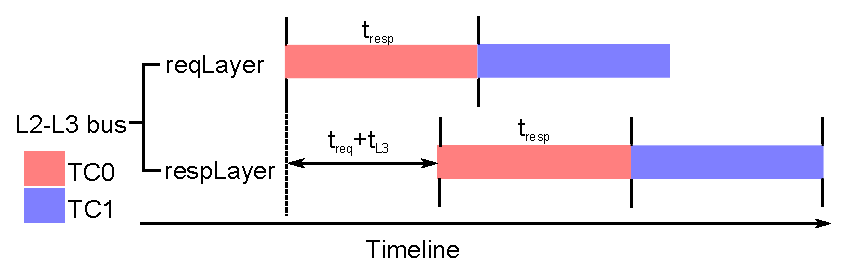
\includegraphics[width=3.2in]{figs/hit_schedule.eps}
        \caption{Cache hit timing path schedule.}
        \label{fig:hit_schedule}
    \end{center}
\end{figure}

Deriving a schedule that is suitable for L2 misses assuming they are followed 
by L3 misses is similar. The turn lengths for both L3-memory bus layers and
the memory controller should be $t_{mem}$, the minimum memory turn length.
Although these bus turns could have been smaller, this would provide no
benefit since they transfer responsesto and from the memory controller exclusively.
The L2-L3 bus layer turn lengths should be
the smallest factor of $t_{mem}$ greater than $t_{resp}$. The L2-L3 bus turn 
lengths are greater than just $t_{resp}$ to improve the schedule's repeatability.
Each device schedule is offset so that it starts when the data is available 
based on the timing of an L2 miss followed by an L3 miss shown 
in~\ref{fig:hit_timing}. Table \ref{tab:l2_miss_schedules} summarizes both the
turn lengths and offsets in this schedule. Here $t_{read}$ is the worst case
memory read time and
$t_{req}^+ = Max(\{n \times t_{mem} | n\in\mathbb{N}, n\times t_{mem} > t_{resp} \})$
As discussed in Section~\ref{sec:eval_coord} we did not find a schedule with 
a lower average L2 miss latency given that it is followed by an L3 miss.

\def\dc{Blue}
\begin{table}
    \caption{Efficient L2 miss schedules by case.}
    \centering
    \begin{tabular}{|r|r|l|l|}
        \hline
        \multicolumn{4}{|l|}{L2 misses followed by L3 hts}\\\hline
        \multicolumn{2}{|l|}{Device Name} & Turn Length & Offset\\\hline
        \multicolumn{2}{|l|}{L2-L3 Req}  & $t_{resp}$ & 0\\\hline
        \multicolumn{2}{|l|}{L2-L3 Resp} & $t_{resp}$ &
          $t_{req}+t_{L3}$\\\hline\hline
        \multicolumn{4}{|l|}{L2 misses followed by L3 hts}\\\hline
        \multicolumn{2}{|l|}{L2-L3 Req}   & $t_{resp}^+$ & 0\\\hline
        \multicolumn{2}{|l|}{L3-Mem Req}  & $t_{mem}$ & $t_{req}+t_{L3}$\\\hline
        \multicolumn{2}{|l|}{Mem Ctl}     & $t_{mem}$ & $2t_{req}+t_{L3}$\\\hline
        \multicolumn{2}{|l|}{L3-Mem Resp} & $t_{mem}$ & 
          $2t_{req}+t_{L3}+t_{read}$\\\hline
        \multicolumn{2}{|l|}{L2-L3 Resp}  & $t_{resp}^+$ &
          $2t_{req}+2t_{L3}+t_{read}+t_{resp}$\\\hline
    \end{tabular}
    \label{tab:l2_miss_schedules}
\end{table}

Scheduling for L2 misses in general, without assuming it is followed by a hit 
or a miss, is much more difficult. Notice that the L2-L3 request and response 
layer turn lengths and the L2-L3 response layer offsets in the efficient 
schedules for the L3 miss and L3 hit cases are different. These differences 
must be balanced for an L2 miss schedule. To ensure repeatability, it is 
unclear if it is preferable to increase the L2-L3 request layer turns to 
$t_{resp}^+$ at the expense of the more common hit case, or if it is better to 
increase the memory controller turn length possibly worsening a bottlneck.
Further, an offset that works well is highly dependant on the actual system 
parameters: $t_{L3}$, $t_{req}$, $t_{resp}$, and $t_{read}$.
We examined this scheduling problem with a simulated annealing optimizer,
and although we could not construct much meaning from the optimal 
schedule, we will show in Section \ref{sec:eval_coord} that the gap between
the best and worst schedules is significant. This suggests that although time 
multiplexing the L2 miss path is a difficult problem, it can greatly impact 
performance.
